% !TEX root =  ../ReplyLetterMain.tex
\clearpage
\section*{Response to 2nd Referee's Comments}
%\newline \newline
We would like to thank the Referee for his/her constructive comments, which have allowed us to considerably improve our paper. The main differences of the new version of the manuscript compared to the previous one can be found in Sections~2, 3 and 5. In addition, changes regarding the specific comments have been made throughout the text.
You may find below our response to the specific issues raised.

%Shared parameter models under random effects misspecification (Dimitris Rizopoulos)
%Latent-model Robustness in JMs for a Primary Endpoint and a Longitudinal Process

\begin{enumerate}
    \item [1,4.] 	
    As the referee noted, the equation for the longitudinal sub-model on page 4 of the original manuscript does not indicate that we used a log transform for PSA levels. This is however the general form of the equation for the longitudinal sub-model, and is only used to introduce the joint model (JM) notation. The actual equation, showing the log transformed PSA levels, baseline covariates and B-spline for the effect of time is Equation (\ref{eq : long_model_prias}) in the original manuscript. That is, it is not the case that the log transformation is used only in simulation study as noted by the referee, but also used for fitting the PRIAS data. 

    Since concerns regarding assumption of normality on errors were also raised by the first referee, we refitted our model with an assumption that the errors are T-distributed (df=3). The residual quantile-quantile plots for the model with normally distributed errors as well as the T-distributed (df=3) errors are shown in Figure \ref{fig : qqplot_norm_t3}. In addition, the fitted marginal $\log_2 \mbox{PSA}$ profiles, and subject specific fitted as well as observed $\log_2 \mbox{PSA}$ profiles of 9 randomly selected patients, using the two different models are presented in Figure \ref{fig : marginal_fitted_psa_NormalVsT3} and Figure \ref{fig : subject_fittedVsObserved_psa_norm_t3}, respectively.

    With regards to the fitted profiles for the 3 demonstration patients, we show their fitted profiles in Figure \ref{fig : fitted_demo_patients_norm_t3}. The fitted profiles are dynamic in nature, and utilize information from both the observed PSA levels and time of latest biopsy. The two time points for each of the patients are the same time points at which we made personalized schedules for these patients in the original manuscript.
    
    \begin{figure}[!htb]
	\centerline{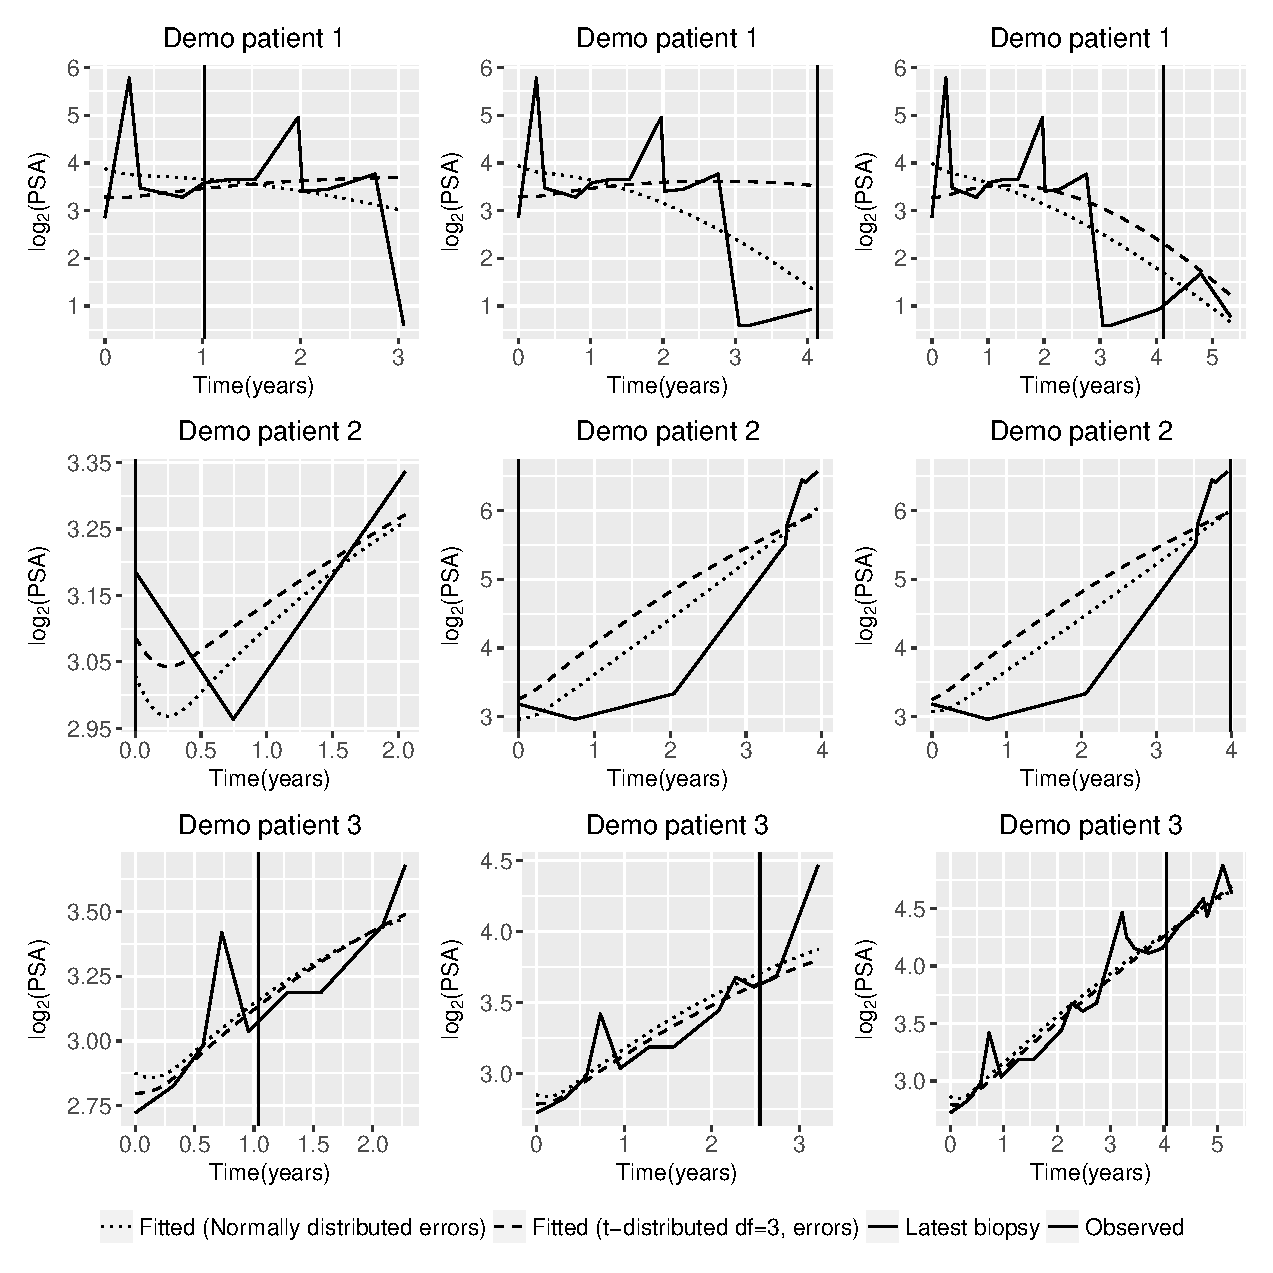
\includegraphics[width=\columnwidth]{images/model_fit/fitted_demo_patients_norm_t3.eps}}
	\caption{Fitted versus observed $\log_2 \mbox{PSA}$ profiles for the three demonstration patients, at two different time points. The vertical line with a dot-dash pattern shows the time of the latest biopsy. The fitted profiles are dynamic in nature, and utilize information from both the observed PSA levels and time of latest biopsy.}
	\label{fig : fitted_demo_patients_norm_t3}
	\end{figure}

    \item[2.] The referee noted that we define $\mathcal{M}_i(t)$ as PSA level up-to last biopsy, and it should not be the case. However on page 5 of the original manuscript it is instead defined as the following:
    \say{$\ldots$ where $\mathcal{M}_i(t) = \{m_i(v), 0\leq v \leq t\}$ denotes the history of the underlying PSA levels up to time $t$}. This is a standard notation can also be found in existing literature \citep{tsiatis2004joint,rizopoulos2012joint}.  

    Regarding the second comment about ability to use historical PSA measurements to make a decision about immediate/delayed biopsy, yes we indeed provide a method to \say{evaluate biopsy time from current time, particularly when there is new information, such as new PSA measure after last biopsy}. To illustrate this, suppose for the $j$-th patient, the last biopsy was conducted at time $t$, and the current visit time at which PSA is measured is $s > t$, then we are interested in finding the time $u > s$ of the next biopsy which utilizes all the available information up to $s$. To this end, all of our approaches are based on the posterior predictive distribution of GR time, given by $p\big\{T^*_j \mid T^*_j > t, \mathcal{Y}_j(s), \mathcal{D}_n\big\}$. Here $\mathcal{Y}_j(s)$ is the history of PSA up to $s$ and the information that no GR was found at last biopsy is included via the condition $T^*_j > t$. Indeed as the referee noted it is possible that $t <T^*_j \leq s$, and then biopsy should be conducted immediately. However, it is often the case that difference between consecutive biopsies is required to be at least an year. Thus even if the schedule also suggests a time $t < u \leq s$, the biopsy should be conducted with a delay of $1 - t$. We have discussed this scenario in Section \ref{subsec : pers_sched_algorithm} of the original manuscript. In addition, we have shown the entire decision making process related to conducting a biopsy in the flowchart in Figure \ref{fig : sched_algorithm} of the original manuscript.
    
    \item[3.] We observed in Figure \ref{fig : prias_demo_pid_911} of the original manuscript that the variance of posterior predictive distribution of event time decreases as more information is gathered over time. That is, a schedule based on expected/median time of Gleason reclassification (GR) is less accurate (the consistency property) in predicting true event time when less information is available. In comparison, the schedule based on dynamic risk of GR is robust in the sense that it is more risk averse than the schedule based on median time of GR (50\% risk), at all time points. For example, in PRIAS, on average it schedules biopsies whenever the risk increases more than 5.3\%. Thus, it is less likely to overshoot the true GR time by a big margin even if less information is available for the patients. This is also demonstrated via the simulation study, wherein the schedule based on dynamic risk of GR leads to almost the same mean offset and variance of offset across the three subgroups of patients. However, given that  the term robust implies a different meaning in a statistical context, we have removed it in the updated manuscript.

\end{enumerate}

\subsection*{Minor Concerns Shared by the 2nd Referee}

\begin{enumerate}
	\item[1.] We have updated the captions of tables and graphs in the updated version of the manuscript.
	\item[2,4.] For the two parameters $\kappa$ and $\eta$ mentioned by the referee, we do not use fixed set of values. We compute the parameter $\kappa$ (dynamic risk of GR) from the data, as shown in Section \ref{subsec : estimation} of the original manuscript. That is, we obviate choosing this value manually. When it is chosen manually, it may not always give the best results. For example, often clinicians use a $\kappa = 0.05$ or 5\% risk, however as shown in \ref{table : sim_study_pooled_estimates_extended} in supplementary material the performance of this schedule is exactly same as that of annual schedule. That is, it gives a very small offset at the cost of too many biopsies. 

	With regards to the choice of weights $\eta_1, \eta_2$, as discussed in Section \ref{subsec : optimal_schedule} of the original manuscript, this choice can be obviated by reformulating the optimization of original weighted sum as a constrained optimization problem. For example, if $\eta_1$ is the weight corresponding to average number of biopsies $E(N^S)$ and $\eta_2$ is the weight corresponding to average offset $E(O^S)$, then we can instead put a constraint $C$ on average offset, and then optimize for only the number of biopsies. Since multiple studies have reported small prostate cancer specific mortality in low risk patients enrolled in active surveillance programs \citep{loeb2016immediate,tosoian2011active,klotz2009clinical},a recommended cutoff $C$ on average offset is 1 year. We have also added this information in the discussion section of the updated manuscript.

	\item[3.] We agree to the referee with regards to not having a direct interpretation of age since we also have quadratic form of age in the model.
YES WE DID A MISTAKE...DID WE? atleast one of the two is significant anyway

 However in the original manuscript we did not interpret the effect size, but rather only mentioned that \say{$\ldots$ and the age at the time of inclusion in AS were strongly associated with the hazard of GR}. This is still true, because both the linear and quadratic effects of age are significant. --WE CALL IT SIGNIFICANT NOW..CHANGE OF SENTENCE

 \item[4.] Good and bad 
\end{enumerate}

